\documentclass{beamer}
\usepackage{physics}
\usepackage{amsmath}
\usepackage{tikz}
\usepackage{mathdots}
\usepackage{yhmath}
\usepackage{cancel}
\usepackage{color}
\usepackage{siunitx}
\usepackage{array}
\usepackage{multirow}
\usepackage[version=4]{mhchem}
\usepackage{amssymb}
\usepackage{textcomp, gensymb}
\usepackage{pifont}
\newcommand{\cmark}{\ding{51}}%
\newcommand{\xmark}{\ding{55}}%
\usepackage{tabularx}
\usepackage{extarrows}
\usepackage{booktabs}
\usetikzlibrary{fadings}
\usetikzlibrary{patterns}
\usetikzlibrary{shadows.blur}
\usetikzlibrary{shapes}
\usepackage[style=verbose,backend=bibtex]{biblatex}
\addbibresource{wannier.bib}
\addbibresource{hubbard.bib}
\renewcommand{\footnotesize}{\scriptsize}
\usepackage{listings}
\usepackage{hyperref}

\newcommand{\pair}[1]{\langle #1 \rangle}
\DeclareMathOperator{\ee}{e}
\DeclareMathOperator{\ii}{i}

\newcommand{\concept}[1]{\textbf{#1}}
\newcommand*{\abinitio}{\textit{ab initio}}
\newcommand{\shortcode}[1]{\texttt{#1}}

%Information to be included in the title page:
\title{Constrained RPA}
\author{Jinyuan Wu}

\usetheme{madrid}

\begin{document}

\frame{\titlepage}

\begin{frame}
\frametitle{Table of contents}

\tableofcontents    

\end{frame}

\section{General idea}

\begin{frame}
\frametitle{Motivation}

Strongly correlated electrons are \dots
\begin{itemize}
    \item Hard to treat \abinitio
    \item Should be described by a lattice model
\end{itemize}    

\begin{equation}
    H = - t \sum_{\pair{\vb*{i}, \vb*{j}}, \sigma}
        c^\dagger_{\vb*{i} \sigma} c_{\vb*{j} \sigma}
        + \text{h.c.}
        + U \sum_{\vb*{i}} n_{\vb*{i} \uparrow} n_{\vb*{i} \downarrow}.
\end{equation}

But should all electrons be included?

\begin{itemize}
    \item $d$ electron: correlated ones 
    \item $r$ electron: ``trivial'' ones
\end{itemize}

\end{frame}

\begin{frame}
\frametitle{Diagrammatics}

Screening by $d$ and $r$ = first screened by $r$ and then $d$

\begin{equation}
    W = (1 - v P)^{-1} v = (1 - W_r P_d)^{-1} W_r, \quad 
    W_r = (1 - v P_r)^{-1} v,
\end{equation}
\begin{itemize}
    \item $W$ is effective interaction 
    \item where $P_d$ is the polarization within $d$ subspace,
    \item and $P_r = P - P_d$
\end{itemize}

\begin{center}
    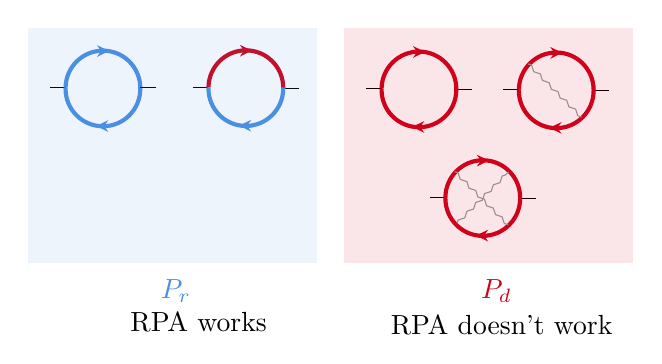
\begin{tikzpicture}[x=0.75pt,y=0.75pt,yscale=-0.6,xscale=0.6]
    %uncomment if require: \path (0,347); %set diagram left start at 0, and has height of 347
    
    %Straight Lines [id:da5540695165355127] 
    \draw    (188.33,140.43) -- (200.75,140.43) ;
    %Straight Lines [id:da04050373051387535] 
    \draw    (260.75,141.18) -- (273.16,141.18) ;
    %Straight Lines [id:da6630274547141346] 
    \draw    (73.58,140.68) -- (86,140.68) ;
    %Shape: Arc [id:dp4109963510412227] 
    \draw  [draw opacity=0][line width=1.5]  (86,140.68) .. controls (86.17,124.26) and (99.54,111) .. (116,111) .. controls (132.52,111) and (145.92,124.36) .. (146,140.86) -- (116,141) -- cycle ; \draw  [color={rgb, 255:red, 74; green, 144; blue, 226 }  ,draw opacity=1 ][line width=1.5]  (86,140.68) .. controls (86.17,124.26) and (99.54,111) .. (116,111) .. controls (132.52,111) and (145.92,124.36) .. (146,140.86) ;  
    %Shape: Arc [id:dp7623323581985462] 
    \draw  [draw opacity=0][line width=1.5]  (145.93,139.9) .. controls (145.96,140.51) and (145.98,141.11) .. (145.98,141.73) .. controls (145.98,158.3) and (132.55,171.73) .. (115.98,171.73) .. controls (99.41,171.73) and (85.98,158.3) .. (85.98,141.73) .. controls (85.98,141.38) and (85.99,141.03) .. (86,140.68) -- (115.98,141.73) -- cycle ; \draw  [color={rgb, 255:red, 74; green, 144; blue, 226 }  ,draw opacity=1 ][line width=1.5]  (145.93,139.9) .. controls (145.96,140.51) and (145.98,141.11) .. (145.98,141.73) .. controls (145.98,158.3) and (132.55,171.73) .. (115.98,171.73) .. controls (99.41,171.73) and (85.98,158.3) .. (85.98,141.73) .. controls (85.98,141.38) and (85.99,141.03) .. (86,140.68) ;  
    %Straight Lines [id:da6949092443253346] 
    \draw [color={rgb, 255:red, 74; green, 144; blue, 226 }  ,draw opacity=1 ]   (116.46,111.27) -- (118,111.26) ;
    \draw [shift={(121,111.25)}, rotate = 179.74] [fill={rgb, 255:red, 74; green, 144; blue, 226 }  ,fill opacity=1 ][line width=0.08]  [draw opacity=0] (9.82,-4.72) -- (0,0) -- (9.82,4.72) -- (6.52,0) -- cycle    ;
    %Straight Lines [id:da20135215487389058] 
    \draw [color={rgb, 255:red, 74; green, 144; blue, 226 }  ,draw opacity=1 ]   (116.96,171.52) -- (113.5,171.51) ;
    \draw [shift={(110.5,171.5)}, rotate = 0.18] [fill={rgb, 255:red, 74; green, 144; blue, 226 }  ,fill opacity=1 ][line width=0.08]  [draw opacity=0] (9.82,-4.72) -- (0,0) -- (9.82,4.72) -- (6.52,0) -- cycle    ;
    %Shape: Arc [id:dp5780798181398437] 
    \draw  [draw opacity=0][line width=1.5]  (200.75,140.43) .. controls (200.92,124.01) and (214.29,110.75) .. (230.75,110.75) .. controls (247.32,110.75) and (260.75,124.18) .. (260.75,140.75) .. controls (260.75,140.9) and (260.75,141.04) .. (260.75,141.18) -- (230.75,140.75) -- cycle ; \draw  [color={rgb, 255:red, 208; green, 2; blue, 27 }  ,draw opacity=1 ][line width=1.5]  (200.75,140.43) .. controls (200.92,124.01) and (214.29,110.75) .. (230.75,110.75) .. controls (247.32,110.75) and (260.75,124.18) .. (260.75,140.75) .. controls (260.75,140.9) and (260.75,141.04) .. (260.75,141.18) ;  
    %Shape: Arc [id:dp4203795619019626] 
    \draw  [draw opacity=0][line width=1.5]  (260.72,140.52) .. controls (260.73,140.84) and (260.73,141.16) .. (260.73,141.48) .. controls (260.73,158.05) and (247.3,171.48) .. (230.73,171.48) .. controls (214.17,171.48) and (200.73,158.05) .. (200.73,141.48) .. controls (200.73,141.13) and (200.74,140.78) .. (200.75,140.43) -- (230.73,141.48) -- cycle ; \draw  [color={rgb, 255:red, 74; green, 144; blue, 226 }  ,draw opacity=1 ][line width=1.5]  (260.72,140.52) .. controls (260.73,140.84) and (260.73,141.16) .. (260.73,141.48) .. controls (260.73,158.05) and (247.3,171.48) .. (230.73,171.48) .. controls (214.17,171.48) and (200.73,158.05) .. (200.73,141.48) .. controls (200.73,141.13) and (200.74,140.78) .. (200.75,140.43) ;  
    %Straight Lines [id:da5601857262824945] 
    \draw [color={rgb, 255:red, 208; green, 2; blue, 27 }  ,draw opacity=1 ]   (231.21,111.02) -- (232.75,111.01) ;
    \draw [shift={(235.75,111)}, rotate = 179.74] [fill={rgb, 255:red, 208; green, 2; blue, 27 }  ,fill opacity=1 ][line width=0.08]  [draw opacity=0] (9.82,-4.72) -- (0,0) -- (9.82,4.72) -- (6.52,0) -- cycle    ;
    %Straight Lines [id:da9251865186613348] 
    \draw [color={rgb, 255:red, 74; green, 144; blue, 226 }  ,draw opacity=1 ]   (231.71,171.27) -- (228.25,171.26) ;
    \draw [shift={(225.25,171.25)}, rotate = 0.18] [fill={rgb, 255:red, 74; green, 144; blue, 226 }  ,fill opacity=1 ][line width=0.08]  [draw opacity=0] (9.82,-4.72) -- (0,0) -- (9.82,4.72) -- (6.52,0) -- cycle    ;
    %Straight Lines [id:da9010174504087856] 
    \draw    (146,140.86) -- (158.42,140.86) ;
    %Straight Lines [id:da9399083659561258] 
    \draw    (327.33,141.43) -- (339.75,141.43) ;
    %Straight Lines [id:da8842581910878855] 
    \draw    (399.75,142.18) -- (412.16,142.18) ;
    %Shape: Arc [id:dp6460550686474504] 
    \draw  [draw opacity=0][line width=1.5]  (339.75,141.43) .. controls (339.92,125.01) and (353.29,111.75) .. (369.75,111.75) .. controls (386.32,111.75) and (399.75,125.18) .. (399.75,141.75) .. controls (399.75,141.9) and (399.75,142.04) .. (399.75,142.18) -- (369.75,141.75) -- cycle ; \draw  [color={rgb, 255:red, 208; green, 2; blue, 27 }  ,draw opacity=1 ][line width=1.5]  (339.75,141.43) .. controls (339.92,125.01) and (353.29,111.75) .. (369.75,111.75) .. controls (386.32,111.75) and (399.75,125.18) .. (399.75,141.75) .. controls (399.75,141.9) and (399.75,142.04) .. (399.75,142.18) ;  
    %Shape: Arc [id:dp011913212107167004] 
    \draw  [draw opacity=0][line width=1.5]  (399.72,141.52) .. controls (399.73,141.84) and (399.73,142.16) .. (399.73,142.48) .. controls (399.73,159.05) and (386.3,172.48) .. (369.73,172.48) .. controls (353.17,172.48) and (339.73,159.05) .. (339.73,142.48) .. controls (339.73,142.13) and (339.74,141.78) .. (339.75,141.43) -- (369.73,142.48) -- cycle ; \draw  [color={rgb, 255:red, 208; green, 2; blue, 27 }  ,draw opacity=1 ][line width=1.5]  (399.72,141.52) .. controls (399.73,141.84) and (399.73,142.16) .. (399.73,142.48) .. controls (399.73,159.05) and (386.3,172.48) .. (369.73,172.48) .. controls (353.17,172.48) and (339.73,159.05) .. (339.73,142.48) .. controls (339.73,142.13) and (339.74,141.78) .. (339.75,141.43) ;  
    %Straight Lines [id:da7976352471721526] 
    \draw [color={rgb, 255:red, 208; green, 2; blue, 27 }  ,draw opacity=1 ]   (370.21,112.02) -- (371.75,112.01) ;
    \draw [shift={(374.75,112)}, rotate = 179.74] [fill={rgb, 255:red, 208; green, 2; blue, 27 }  ,fill opacity=1 ][line width=0.08]  [draw opacity=0] (9.82,-4.72) -- (0,0) -- (9.82,4.72) -- (6.52,0) -- cycle    ;
    %Straight Lines [id:da3119516972821752] 
    \draw [color={rgb, 255:red, 208; green, 2; blue, 27 }  ,draw opacity=1 ]   (370.71,172.27) -- (367.25,172.26) ;
    \draw [shift={(364.25,172.25)}, rotate = 0.18] [fill={rgb, 255:red, 208; green, 2; blue, 27 }  ,fill opacity=1 ][line width=0.08]  [draw opacity=0] (9.82,-4.72) -- (0,0) -- (9.82,4.72) -- (6.52,0) -- cycle    ;
    %Straight Lines [id:da6292473305470048] 
    \draw    (437.58,142.18) -- (450,142.18) ;
    %Straight Lines [id:da4502338075251966] 
    \draw    (510,142.93) -- (522.41,142.93) ;
    %Shape: Arc [id:dp969117541936845] 
    \draw  [draw opacity=0][line width=1.5]  (450,142.18) .. controls (450.17,125.76) and (463.54,112.5) .. (480,112.5) .. controls (496.57,112.5) and (510,125.93) .. (510,142.5) .. controls (510,142.65) and (510,142.79) .. (510,142.93) -- (480,142.5) -- cycle ; \draw  [color={rgb, 255:red, 208; green, 2; blue, 27 }  ,draw opacity=1 ][line width=1.5]  (450,142.18) .. controls (450.17,125.76) and (463.54,112.5) .. (480,112.5) .. controls (496.57,112.5) and (510,125.93) .. (510,142.5) .. controls (510,142.65) and (510,142.79) .. (510,142.93) ;  
    %Shape: Arc [id:dp5229621002109612] 
    \draw  [draw opacity=0][line width=1.5]  (509.97,142.27) .. controls (509.98,142.59) and (509.98,142.91) .. (509.98,143.23) .. controls (509.98,159.8) and (496.55,173.23) .. (479.98,173.23) .. controls (463.42,173.23) and (449.98,159.8) .. (449.98,143.23) .. controls (449.98,142.88) and (449.99,142.53) .. (450,142.18) -- (479.98,143.23) -- cycle ; \draw  [color={rgb, 255:red, 208; green, 2; blue, 27 }  ,draw opacity=1 ][line width=1.5]  (509.97,142.27) .. controls (509.98,142.59) and (509.98,142.91) .. (509.98,143.23) .. controls (509.98,159.8) and (496.55,173.23) .. (479.98,173.23) .. controls (463.42,173.23) and (449.98,159.8) .. (449.98,143.23) .. controls (449.98,142.88) and (449.99,142.53) .. (450,142.18) ;  
    %Straight Lines [id:da27859309067037596] 
    \draw [color={rgb, 255:red, 208; green, 2; blue, 27 }  ,draw opacity=1 ]   (480.46,112.77) -- (482,112.76) ;
    \draw [shift={(485,112.75)}, rotate = 179.74] [fill={rgb, 255:red, 208; green, 2; blue, 27 }  ,fill opacity=1 ][line width=0.08]  [draw opacity=0] (9.82,-4.72) -- (0,0) -- (9.82,4.72) -- (6.52,0) -- cycle    ;
    %Straight Lines [id:da032744621306240784] 
    \draw [color={rgb, 255:red, 208; green, 2; blue, 27 }  ,draw opacity=1 ]   (480.96,173.02) -- (477.5,173.01) ;
    \draw [shift={(474.5,173)}, rotate = 0.18] [fill={rgb, 255:red, 208; green, 2; blue, 27 }  ,fill opacity=1 ][line width=0.08]  [draw opacity=0] (9.82,-4.72) -- (0,0) -- (9.82,4.72) -- (6.52,0) -- cycle    ;
    %Straight Lines [id:da6710684020883058] 
    \draw [color={rgb, 255:red, 155; green, 155; blue, 155 }  ,draw opacity=1 ]   (457.49,121.7) .. controls (459.85,121.7) and (461.03,122.88) .. (461.03,125.24) .. controls (461.03,127.6) and (462.21,128.78) .. (464.57,128.77) .. controls (466.93,128.77) and (468.11,129.95) .. (468.1,132.31) .. controls (468.1,134.67) and (469.28,135.85) .. (471.64,135.85) .. controls (473.99,135.85) and (475.17,137.03) .. (475.17,139.38) .. controls (475.17,141.74) and (476.35,142.92) .. (478.71,142.92) .. controls (481.06,142.92) and (482.24,144.1) .. (482.24,146.45) .. controls (482.24,148.81) and (483.42,149.99) .. (485.78,149.99) .. controls (488.13,149.99) and (489.31,151.17) .. (489.31,153.52) .. controls (489.31,155.88) and (490.49,157.06) .. (492.85,157.06) .. controls (495.21,157.05) and (496.39,158.23) .. (496.39,160.59) .. controls (496.38,162.95) and (497.56,164.13) .. (499.92,164.13) -- (500.25,164.46) -- (500.25,164.46) ;
    %Straight Lines [id:da6332371972741615] 
    \draw    (378.58,228.68) -- (391,228.68) ;
    %Straight Lines [id:da518138397790002] 
    \draw    (451,229.43) -- (463.41,229.43) ;
    %Shape: Arc [id:dp7737420651474474] 
    \draw  [draw opacity=0][line width=1.5]  (391,228.68) .. controls (391.17,212.26) and (404.54,199) .. (421,199) .. controls (437.57,199) and (451,212.43) .. (451,229) .. controls (451,229.15) and (451,229.29) .. (451,229.43) -- (421,229) -- cycle ; \draw  [color={rgb, 255:red, 208; green, 2; blue, 27 }  ,draw opacity=1 ][line width=1.5]  (391,228.68) .. controls (391.17,212.26) and (404.54,199) .. (421,199) .. controls (437.57,199) and (451,212.43) .. (451,229) .. controls (451,229.15) and (451,229.29) .. (451,229.43) ;  
    %Shape: Arc [id:dp5679501089367622] 
    \draw  [draw opacity=0][line width=1.5]  (450.97,228.77) .. controls (450.98,229.09) and (450.98,229.41) .. (450.98,229.73) .. controls (450.98,246.3) and (437.55,259.73) .. (420.98,259.73) .. controls (404.42,259.73) and (390.98,246.3) .. (390.98,229.73) .. controls (390.98,229.38) and (390.99,229.03) .. (391,228.68) -- (420.98,229.73) -- cycle ; \draw  [color={rgb, 255:red, 208; green, 2; blue, 27 }  ,draw opacity=1 ][line width=1.5]  (450.97,228.77) .. controls (450.98,229.09) and (450.98,229.41) .. (450.98,229.73) .. controls (450.98,246.3) and (437.55,259.73) .. (420.98,259.73) .. controls (404.42,259.73) and (390.98,246.3) .. (390.98,229.73) .. controls (390.98,229.38) and (390.99,229.03) .. (391,228.68) ;  
    %Straight Lines [id:da05355660373437332] 
    \draw [color={rgb, 255:red, 208; green, 2; blue, 27 }  ,draw opacity=1 ]   (421.46,199.27) -- (423,199.26) ;
    \draw [shift={(426,199.25)}, rotate = 179.74] [fill={rgb, 255:red, 208; green, 2; blue, 27 }  ,fill opacity=1 ][line width=0.08]  [draw opacity=0] (9.82,-4.72) -- (0,0) -- (9.82,4.72) -- (6.52,0) -- cycle    ;
    %Straight Lines [id:da8830335731017662] 
    \draw [color={rgb, 255:red, 208; green, 2; blue, 27 }  ,draw opacity=1 ]   (421.96,259.52) -- (418.5,259.51) ;
    \draw [shift={(415.5,259.5)}, rotate = 0.18] [fill={rgb, 255:red, 208; green, 2; blue, 27 }  ,fill opacity=1 ][line width=0.08]  [draw opacity=0] (9.82,-4.72) -- (0,0) -- (9.82,4.72) -- (6.52,0) -- cycle    ;
    %Straight Lines [id:da23096666699581192] 
    \draw [color={rgb, 255:red, 155; green, 155; blue, 155 }  ,draw opacity=1 ]   (398.49,208.2) .. controls (400.85,208.2) and (402.03,209.38) .. (402.03,211.74) .. controls (402.03,214.1) and (403.21,215.28) .. (405.57,215.27) .. controls (407.93,215.27) and (409.11,216.45) .. (409.1,218.81) .. controls (409.1,221.17) and (410.28,222.35) .. (412.64,222.35) .. controls (414.99,222.35) and (416.17,223.53) .. (416.17,225.88) .. controls (416.17,228.24) and (417.35,229.42) .. (419.71,229.42) .. controls (422.06,229.42) and (423.24,230.6) .. (423.24,232.95) .. controls (423.24,235.31) and (424.42,236.49) .. (426.78,236.49) .. controls (429.13,236.49) and (430.31,237.67) .. (430.31,240.02) .. controls (430.31,242.38) and (431.49,243.56) .. (433.85,243.56) .. controls (436.21,243.55) and (437.39,244.73) .. (437.39,247.09) .. controls (437.38,249.45) and (438.56,250.63) .. (440.92,250.63) -- (441.25,250.96) -- (441.25,250.96) ;
    %Straight Lines [id:da6651557300213262] 
    \draw [color={rgb, 255:red, 155; green, 155; blue, 155 }  ,draw opacity=1 ]   (400.33,249.67) .. controls (400.32,247.32) and (401.5,246.14) .. (403.86,246.14) .. controls (406.22,246.14) and (407.4,244.96) .. (407.4,242.6) .. controls (407.4,240.25) and (408.58,239.07) .. (410.93,239.07) .. controls (413.29,239.07) and (414.47,237.89) .. (414.47,235.53) .. controls (414.47,233.18) and (415.65,232) .. (418,232) .. controls (420.36,232) and (421.54,230.82) .. (421.54,228.46) .. controls (421.54,226.11) and (422.72,224.93) .. (425.07,224.93) .. controls (427.43,224.93) and (428.61,223.75) .. (428.61,221.39) .. controls (428.61,219.03) and (429.79,217.85) .. (432.15,217.85) .. controls (434.5,217.85) and (435.68,216.67) .. (435.68,214.32) .. controls (435.68,211.96) and (436.86,210.78) .. (439.22,210.78) -- (441.67,208.33) -- (441.67,208.33) ;
    %Shape: Rectangle [id:dp42077016684860147] 
    \draw  [draw opacity=0][fill={rgb, 255:red, 74; green, 144; blue, 226 }  ,fill opacity=0.1 ] (56,93) -- (287.83,93) -- (287.83,281.52) -- (56,281.52) -- cycle ;
    %Shape: Rectangle [id:dp16340916001575945] 
    \draw  [draw opacity=0][fill={rgb, 255:red, 208; green, 2; blue, 27 }  ,fill opacity=0.1 ] (309.83,93) -- (541.67,93) -- (541.67,281.52) -- (309.83,281.52) -- cycle ;
    
    % Text Node
    \draw (431.92,293) node [anchor=north] [inner sep=0.75pt]  [color={rgb, 255:red, 208; green, 2; blue, 27 }  ,opacity=1 ]  {$P_{d}$};
    % Text Node
    \draw (174.5,293) node [anchor=north] [inner sep=0.75pt]  [color={rgb, 255:red, 74; green, 144; blue, 226 }  ,opacity=1 ]  {$P_{r}$};
    % Text Node
    \draw (345,321) node [anchor=north west][inner sep=0.75pt]   [align=left] {RPA doesn't work};
    % Text Node
    \draw (136,319.33) node [anchor=north west][inner sep=0.75pt]   [align=left] {RPA works};
    
    
    \end{tikzpicture}
    
\end{center}

\end{frame}

\begin{frame}
\frametitle{Diagrammatics}

\begin{itemize}
    \item $P_d$ hard to obtain $\Rightarrow$ we left it to an effective interaction 
    without doing resummation for it
    \item $P_r$ can be done by \shortcode{epsilon} $\Rightarrow$
        $W_r$ can be obtained by \shortcode{epsilon}
    \item But 
    \begin{center}
        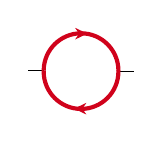
\begin{tikzpicture}[x=0.75pt,y=0.75pt,yscale=-0.6,xscale=0.6]
            %uncomment if require: \path (0,300); %set diagram left start at 0, and has height of 300
            
            %Straight Lines [id:da24436922749346324] 
            \draw    (347.33,149.91) -- (359.75,149.91) ;
            %Straight Lines [id:da2754743780079656] 
            \draw    (419.75,150.66) -- (432.16,150.66) ;
            %Shape: Arc [id:dp8646599824167052] 
            \draw  [draw opacity=0][line width=1.5]  (359.75,149.91) .. controls (359.92,133.49) and (373.29,120.23) .. (389.75,120.23) .. controls (406.32,120.23) and (419.75,133.66) .. (419.75,150.23) .. controls (419.75,150.37) and (419.75,150.52) .. (419.75,150.66) -- (389.75,150.23) -- cycle ; \draw  [color={rgb, 255:red, 208; green, 2; blue, 27 }  ,draw opacity=1 ][line width=1.5]  (359.75,149.91) .. controls (359.92,133.49) and (373.29,120.23) .. (389.75,120.23) .. controls (406.32,120.23) and (419.75,133.66) .. (419.75,150.23) .. controls (419.75,150.37) and (419.75,150.52) .. (419.75,150.66) ;  
            %Shape: Arc [id:dp0010091790996433758] 
            \draw  [draw opacity=0][line width=1.5]  (419.72,150) .. controls (419.73,150.32) and (419.73,150.64) .. (419.73,150.96) .. controls (419.73,167.53) and (406.3,180.96) .. (389.73,180.96) .. controls (373.17,180.96) and (359.73,167.53) .. (359.73,150.96) .. controls (359.73,150.61) and (359.74,150.26) .. (359.75,149.91) -- (389.73,150.96) -- cycle ; \draw  [color={rgb, 255:red, 208; green, 2; blue, 27 }  ,draw opacity=1 ][line width=1.5]  (419.72,150) .. controls (419.73,150.32) and (419.73,150.64) .. (419.73,150.96) .. controls (419.73,167.53) and (406.3,180.96) .. (389.73,180.96) .. controls (373.17,180.96) and (359.73,167.53) .. (359.73,150.96) .. controls (359.73,150.61) and (359.74,150.26) .. (359.75,149.91) ;  
            %Straight Lines [id:da4499744987871399] 
            \draw [color={rgb, 255:red, 208; green, 2; blue, 27 }  ,draw opacity=1 ]   (390.21,120.5) -- (391.75,120.49) ;
            \draw [shift={(394.75,120.48)}, rotate = 179.74] [fill={rgb, 255:red, 208; green, 2; blue, 27 }  ,fill opacity=1 ][line width=0.08]  [draw opacity=0] (9.82,-4.72) -- (0,0) -- (9.82,4.72) -- (6.52,0) -- cycle    ;
            %Straight Lines [id:da7286267028918754] 
            \draw [color={rgb, 255:red, 208; green, 2; blue, 27 }  ,draw opacity=1 ]   (390.71,180.75) -- (387.25,180.74) ;
            \draw [shift={(384.25,180.73)}, rotate = 0.18] [fill={rgb, 255:red, 208; green, 2; blue, 27 }  ,fill opacity=1 ][line width=0.08]  [draw opacity=0] (9.82,-4.72) -- (0,0) -- (9.82,4.72) -- (6.52,0) -- cycle    ; 
            \end{tikzpicture}            
    \end{center}
    is not in $P_r$, or otherwise we have double counting
    \item That's what we call \concept{constrained RPA (cRPA)}
    \item A program to calculate a single ring diagram is needed
\end{itemize}

\end{frame}

\begin{frame}
\frametitle{Band part}

In $GW$:

\begin{equation}
    \begin{aligned}
        \varepsilon^{GW} &= \varepsilon^0 + \Sigma^{\text{Hartree}} + \Sigma^{GW} \\
        &= \underbrace{\varepsilon^0 + \Sigma^{\text{Hartree}} + V^{\text{xc}}}_{\text{\shortcode{WFN}}} 
        + \underbrace{\Sigma^{GW}}_{\text{\shortcode{sigma}}} 
        - \underbrace{V^{\text{xc}}}_{\text{\shortcode{vxc.dat}}}
    \end{aligned}
\end{equation}

In the effective model \dots
\begin{itemize}
    \item We want $\varepsilon^0$ 
    \item So the same $-V^{\text{xc}}$ procedure is needed
    \item A problem to calculate a single ring diagram is needed.
\end{itemize}

\end{frame}

\begin{frame}
\frametitle{Risks in accuracy}

Uncontrolled approximation: does RPA work for 
\begin{center}
    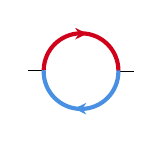
\begin{tikzpicture}[x=0.75pt,y=0.75pt,yscale=-0.6,xscale=0.6]
        %uncomment if require: \path (0,300); %set diagram left start at 0, and has height of 300
        
        %Straight Lines [id:da24436922749346324] 
        \draw    (347.33,149.91) -- (359.75,149.91) ;
        %Straight Lines [id:da2754743780079656] 
        \draw    (419.75,150.66) -- (432.16,150.66) ;
        %Shape: Arc [id:dp8646599824167052] 
        \draw  [draw opacity=0][line width=1.5]  (359.75,149.91) .. controls (359.92,133.49) and (373.29,120.23) .. (389.75,120.23) .. controls (406.32,120.23) and (419.75,133.66) .. (419.75,150.23) .. controls (419.75,150.37) and (419.75,150.52) .. (419.75,150.66) -- (389.75,150.23) -- cycle ; \draw  [color={rgb, 255:red, 208; green, 2; blue, 27 }  ,draw opacity=1 ][line width=1.5]  (359.75,149.91) .. controls (359.92,133.49) and (373.29,120.23) .. (389.75,120.23) .. controls (406.32,120.23) and (419.75,133.66) .. (419.75,150.23) .. controls (419.75,150.37) and (419.75,150.52) .. (419.75,150.66) ;  
        %Shape: Arc [id:dp0010091790996433758] 
        \draw  [draw opacity=0][line width=1.5]  (419.72,150) .. controls (419.73,150.32) and (419.73,150.64) .. (419.73,150.96) .. controls (419.73,167.53) and (406.3,180.96) .. (389.73,180.96) .. controls (373.17,180.96) and (359.73,167.53) .. (359.73,150.96) .. controls (359.73,150.61) and (359.74,150.26) .. (359.75,149.91) -- (389.73,150.96) -- cycle ; \draw  [color={rgb, 255:red, 74; green, 144; blue, 226 }  ,draw opacity=1 ][line width=1.5]  (419.72,150) .. controls (419.73,150.32) and (419.73,150.64) .. (419.73,150.96) .. controls (419.73,167.53) and (406.3,180.96) .. (389.73,180.96) .. controls (373.17,180.96) and (359.73,167.53) .. (359.73,150.96) .. controls (359.73,150.61) and (359.74,150.26) .. (359.75,149.91) ;  
        %Straight Lines [id:da4499744987871399] 
        \draw [color={rgb, 255:red, 208; green, 2; blue, 27 }  ,draw opacity=1 ]   (390.21,120.5) -- (391.75,120.49) ;
        \draw [shift={(394.75,120.48)}, rotate = 179.74] [fill={rgb, 255:red, 208; green, 2; blue, 27 }  ,fill opacity=1 ][line width=0.08]  [draw opacity=0] (9.82,-4.72) -- (0,0) -- (9.82,4.72) -- (6.52,0) -- cycle    ;
        %Straight Lines [id:da7286267028918754] 
        \draw [color={rgb, 255:red, 74; green, 144; blue, 226 }  ,draw opacity=1 ]   (390.71,180.75) -- (387.25,180.74) ;
        \draw [shift={(384.25,180.73)}, rotate = 0.18] [fill={rgb, 255:red, 74; green, 144; blue, 226 }  ,fill opacity=1 ][line width=0.08]  [draw opacity=0] (9.82,-4.72) -- (0,0) -- (9.82,4.72) -- (6.52,0) -- cycle    ;
        \end{tikzpicture}        
\end{center}

The hopping between $d$ electrons is small $\Rightarrow$ it's safe to do so 
\footcite{aryasetiawan2004frequency}

\end{frame}

\section{The problem of dynamic Hubbard model}

\begin{frame}
\frametitle{Dynamic interaction in Hubbard model}

Recall that $W = W(\vb*{r}, \vb*{r}, \textcolor{red}{\omega} )$
$\Rightarrow$ 
$U_{\vb*{i} \vb*{j} \vb*{k} \vb*{l}}(\omega)$
$\Rightarrow$
retarded interaction! 

\begin{itemize}
    \item Hamiltonian form: interactions are always immediate 
    (bosonic auxiliary field required to create retardation)
    \item \dots or path integral formalism is to be used 
    \item Either it, it's slow!!! 
\end{itemize}

\end{frame}

\begin{frame}
\frametitle{Dynamic interaction in Hubbard model}

Is it possible to just enforce $\omega = 0$ \dots
But it's not accurate!\footcite{aryasetiawan2004frequency}

\begin{center}
    \includegraphics[width=0.45\textwidth]{plots/ni-re-sigma-1.PNG}
    \includegraphics[width=0.45\textwidth]{plots/ni-im-sigma-1.PNG}
\end{center}

\ce{Ni} self-energy, from static Hubbard $U = W_r(\omega = 0)$,
and from full $W(\omega)$ 

\end{frame}

\begin{frame}
\frametitle{Dynamic interaction in Hubbard model}

\textbf{Why $\Im \Sigma$ is better captured by static $U$ than $\Re \Sigma$?}

Because $\Im \Sigma \propto \text{DOS}$ TODO: why??

And then high-frequency electrons contribute to low-frequency $\Re \Sigma$ 

\end{frame}

\begin{frame}
\frametitle{Possible way to make the Hubbard model static}

\textbf{Key point: correct the single-electron Hamiltonian using the retarded interaction}

\begin{itemize}
    \item Def: $G_d$ = Green function for $d$ electrons; 
        $\tilde{G}_d$ = Green function for $d$ electrons corrected by $W - W_d$; 
        $W$ = RPA screened Coulomb interaction; 
        $W_d$ = static Hubbard $U$ screened by $G_d$; 
        $\tilde{W}_d$ = static Hubbard $U$ screened by $\tilde{G}_d$;
    \item Ignoring hopping between $d$ and $r$ subspaces caused by $W$
        (so the $\ii W (G - G_d)$ term is irrelevant for $d$ electrons), we have 
        \begin{equation}
            \tilde{G}_d^{-1} - \ii \tilde{G}_d \tilde{W}_d = 
            G_d^{-1} - \ii G_d W_d - \ii G_d (W - W_d).
        \end{equation}
    \item  From
    \begin{equation}
        W = (1 - UP)^{-1} U, \quad P = - \ii G G \Rightarrow
        G^{-1} - \ii GW = (1 - UP)^{-1} G^{-1} 
    \end{equation} 
    we get the final equation: 
    (here $\tilde{P}_d = - \ii \tilde{G}_d \tilde{G}_d$, 
    $P_d = - \ii G_d G_d$)
    \begin{equation}
            (1 - U \tilde{P}_d)^{-1} \tilde{G}_d^{-1}
            = (1 - U P_d^{-1})^{-1} G_d^{-1}
            - \ii G_d  (W -W_d).
        \end{equation}
\end{itemize}

\end{frame}

\section{Existing implementations}

\begin{frame}
\frametitle{Existing implementations}

\begin{itemize}
    \item \textbf{VASP}    
    \shortcode{ALGO=CRPA} selects constrained RPA calculations, 
    available as of VASP.6.4
    \item \textbf{ABINIT} 
    \shortcode{ucrpa} before version 9, 
    as an option in \href{https://docs.abinit.org/variables/gw/\#ucrpa}{the RPA module}
    \item \textbf{BerkeleyGW} \xmark Unfortunately \dots
\end{itemize}

\end{frame}

\end{document}